% System and method. Sources: docs/SYSTEM_ARCHITECTURE.md, scripts/ml/{onset_forecast,
% planner,online_planner,altitude_bandit,geo_features}.py, scripts/adaptive_uplink_cap.py
\section{System and Method}
\label{sec:method}

The management stack has three loops at three time scales
(Fig.~\ref{fig:arch}): a per-robot uplink cap that reacts within a second
(Section~\ref{sec:cap}), a liveness monitor that checks every 20\,s that each
UE process is alive (Section~\ref{sec:dead}), and a terrain-blind learning
layer that decides every 30\,s where the UAV goes (Section~\ref{sec:layer}).
The inner loops keep the managed system sound; the outer loop optimises it.

\subsection{Platform}
\label{sec:platform}
The managed system is the protocol-in-the-loop testbed
of~\cite{makhubela2026satnac}, extended from two to four robots
(Fig.~\ref{fig:arch}). An OpenAirInterface (OAI)~\cite{nikaein2014oai} gNB and
four OAI UEs run over the OAI radio simulator and register to an
Open5GS~\cite{open5gs} core (OAI commit 09c9bb998f). The cell uses band n78 at
3.32\,GHz with 106 resource blocks at 30\,kHz spacing (40\,MHz) and a 5-ms
time-division pattern of five downlink and four uplink slots; every simulated
channel is additive white Gaussian noise (AWGN), so there is no multipath. Each UE's virtual network (TUN) interface sits in its own Linux
network namespace, so robot traffic crosses the real 5G user plane. Gazebo
moves the UAV and four ground robots; a bridge reads their poses every 0.5\,s
and writes a terrain-specific air-to-ground path loss into each UE's channel:
free-space loss with an elevation-dependent line-of-sight
term~\cite{alhourani2014modeling}, plus foliage~\cite{weissberger1982},
diffraction~\cite{itup526} or building loss by terrain, and correlated
shadowing~\cite{gudmundson1991} (details in~\cite{makhubela2026satnac}). A
watchdog relaunches a UE whose process exits after radio-link failure.

\begin{figure*}[t]
\centering
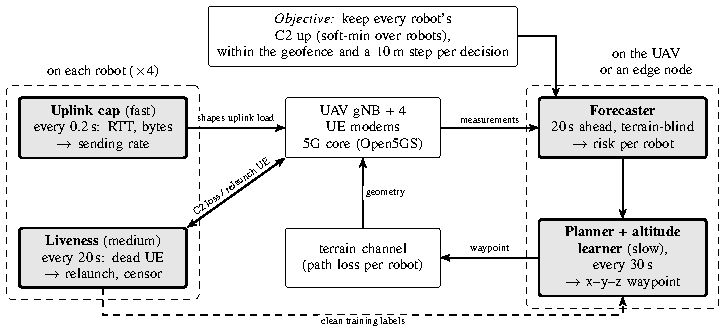
\includegraphics[width=0.82\textwidth]{fig_arch.pdf}
\caption{Management architecture, deployment view: three loops at three time
scales around the managed cell. The cap and the liveness monitor would run on
each robot, the learning layer on the UAV or an edge node; in the testbed all
run on one host. The liveness monitor also cleans the labels the learning layer
is trained on.}
\label{fig:arch}
\end{figure*}

\subsection{Liveness Monitor and Measurement Integrity}
\label{sec:dead}
In OAI, a radio-link failure terminates the UE process, after which the
robot's C2 stays down whatever the UAV does. The liveness monitor probes each
robot's C2 every 20\,s. After 90\,s of total C2 loss it checks the uplink from
inside the robot's namespace and, if the UE is gone, relaunches that UE alone,
giving up after three failed attempts.

The same failure contaminates data recorded before the monitor worked. Once a
UE process dies, the gNB's per-UE counters freeze, and the cycles are logged as
link failures although they record a dead process; a model with lagged
features spots them trivially (the change in block error rate is exactly zero).
We flag a cycle as dead when, for at least three consecutive cycles, the gNB
counters \texttt{dl\_bler}, \texttt{ul\_nb\_rbs} and \texttt{ul\_bits\_per\_sym}
are bit-identical to the previous cycle \emph{and} C2 is down. Frozen counters
on a working link are a quiet cycle, and a failed cycle with moving counters is
a real degradation, so both conditions are required. The rule flags 12.4\,\%
of all cycles and 72.2\,\% of hills failure labels (Table~\ref{tab:a1}), and
flagged cycles are censored. Checked against the monitor's own record of dead or
relaunching UEs, in the 29 of 80 robot series where the monitor was running,
85\,\% of the rule's flags agree, but the rule finds only 56\,\% of the dead
cycles the monitor saw, so some contamination remains in the older data.
% A4: dead_process_extent.csv; rule: onset_forecast.py dead_ue_mask (FREEZE_MIN);
% validation: logs/ml/dead_process_validation.csv; monitor constants: auto_patrol.py RLF_CONFIRM_S, WATCHDOG_PERIOD_S, RLF_MAX_FAILURES

\subsection{Terrain-Blind Learning Layer}
\label{sec:layer}
\textit{Forecaster.} The label is the onset of C2 failure: for a robot whose C2
is up at time $t$, is it down at $t+20$\,s? C2 is up when fewer than 50\,\% of
its probes are lost. Features are UAV--robot geometry, gNB-side link
adaptation and error statistics, and the last commanded move, each with lags,
differences and rolling statistics within one robot's series (65 features).
Three inputs are forbidden: the simulator's injected path loss, the computed
received power (algebraically equivalent to it), and any terrain label. A guard
function checks every feature matrix before it reaches an estimator. Models are
trained leave-one-terrain-out, with thresholds and calibration chosen on an
inner time split of the training terrains.

\textit{Planner.} Each 30-s decision, the planner scores candidate UAV
positions (absolute altitudes 25--55\,m in 5\,m steps, crossed with lateral
offsets of 0 or 15\,m) by a soft minimum over the robots' predicted risks,
$J(u) = \beta^{-1}\log\sum_i e^{\beta r_i(u)}$ with $\beta = 10$, so the
worst-served robot dominates. It moves toward the minimiser at most 10\,m in
altitude per decision. The planner's risk model is the same logistic
regression with spline terms on altitude, distances and elevation angle and
Platt calibration (pooled held-out area under the receiver operating
characteristic curve, ROC-AUC, 0.659). In every fly-off the
planner uses the model trained on the other three terrains, never on the
terrain it flies over.

\textit{Altitude learner.} Because the model cannot choose altitude
(Section~\ref{sec:r-flip}), altitude is learned during the mission. The learner
holds an incumbent altitude and rewards each altitude by the fraction of robots
with C2 up. Its estimates are time-blocked (240\,s blocks), so only comparisons
made close in time count. Every few decisions it probes a neighbouring altitude
($\pm$5 or 10\,m), and it moves when the lower confidence bound of the
neighbour-minus-incumbent difference is above zero ($z = 0.5$). The
\emph{cautious} variant adds a home altitude, the hover altitude of 40\,m: a
move further from home must clear 1.5 standard errors \emph{and} a 0.02 gain,
a move back toward home only the normal bar, and probes are rarer (every 4th
decision, every 20th once all neighbours are worse).
% planner.py (Z_TARGETS, DXY_R, MAX_DZ_STEP, beta=10); altitude_bandit.py AltitudeProber; online_planner.py CAUTIOUS

\subsection{Delay-Adaptive Uplink Cap}
\label{sec:cap}
The cap moves the bottleneck from the UE into the robot's kernel, where it can
be bounded and prioritised, and lets its rate follow the link. It needs no
change to the RAN or core. On each robot's TUN interface, a hierarchical token bucket (HTB) shaper has a
ceiling equal to the cap $c$. C2 and ping (ICMP) traffic use a high-priority class with a
20-packet queue; video uses a low-priority class with a 10-packet queue, so
excess video is dropped rather than buffered. Each robot pings the core every
0.2\,s. ICMP bypasses the kernel video queue, so its round-trip time (RTT) rises only when the
UE's own buffer backs up. With $r_0$ the minimum RTT over 60\,s and $\tilde r$
the median over the last second, Algorithm~\ref{alg:cap} runs every 0.2\,s.
The ``in use'' test keeps an idle robot's cap from rising and then overloading
the link when video resumes. The controller re-creates the shaper when a UE
reattaches with a new TUN. Its only inputs, RTT and bytes sent, are available
on real hardware.

\begin{algorithm}[t]
\caption{Per-Robot Uplink Cap (Every 0.2\,s)}
\label{alg:cap}
\begin{algorithmic}[1]
\small
\STATE initially $c \leftarrow 200$\,kb/s, $\mathit{slow} \leftarrow$ true
\IF{$\tilde r > r_0 + 150$\,ms \OR no reply for 1\,s}
  \STATE $c \leftarrow \max(50,\,0.7c)$; $\mathit{slow} \leftarrow$ false; hold 2\,s
\ELSIF{$\tilde r < r_0 + 50$\,ms \AND sent $\ge 0.7c$ \AND 2\,s since last raise}
  \STATE $c \leftarrow \min(1600,\ \mathit{slow}\ ?\ 2c : c + 50)$
\ENDIF
\end{algorithmic}
\end{algorithm}
% adaptive_uplink_cap.py constants: LO,HI,START=50,1600,200; CUT .7; STEP 50; HOLD 2; UP_EVERY 2; HIGH 150; LOW 50; BASE_WIN 60
